\chapter{正交性}
将列向量看做矩阵,则向量$v$和$w$的内积可以看做$v\cdot w = v\tp w.$
\begin{definition}{向量的正交}{vector orthogonal}
	若$v\tp w=0$,则称$v$和$w$正交(orthogonal)。
\end{definition}
依定义,0和所有向量正交。
\begin{theorem}{正交的模}{}
	若$v,w$正交,则
	\begin{align}
		\norm v^2+\norm w^2=\norm{v+w}^2.
	\end{align}
\end{theorem}
\section{正交性}
\begin{definition}{子空间的正交}{subspace orthogonal}
	定义线性空间$L$的两个子空间$V,W$正交,若$V$中的每一个向量均和$W$中每一个向量正交。
\end{definition}
显然,若$L$的子空间$V,W$正交,则
\begin{align}
	\dim(L)\geqslant\dim(V)+\dim(W).
\end{align}
\begin{definition}{正交补}{orthogonal complement}
	子空间$V$的正交补(orthogonal complement)~$V^\perp$由所有同$V$正交的向量组成。
\end{definition}
只有0同时属于$V$和$V^\perp$。
\begin{theorem}{线性代数基本定理·二}{fundamental theorems of linear algebra II}
	在$\RR^n$中,$\N(A)=\C(A\tp)^\perp.$

	在$\RR^m$中,$\N(A\tp)=\C(A)^\perp.$
\end{theorem}
\begin{theorem}{分解}{resolve}
$\forall x\in\RR^n$均可以分解成
\[
	x=x_\mathrm r+x_\mathrm n,
\]
其中$x_\mathrm r\in\C(A\tp),\enspace x_\mathrm n\in\N(A)$,且这种分解是唯一的。
\end{theorem}
\begin{proof}
	由
	\[
		Ax=A(x_\mathrm r+x_\mathrm n)=Ax_\mathrm r\in\C(A\tp)
	\]
	知,只需证明:
	$\forall b\in\C(A\tp)$,存在唯一的$x_\mathrm r\in\C(A\tp)$使得$Ax_\mathrm r=b.$
	
	若存在$x_\mathrm r,x_\mathrm r'\in\C(A\tp)$满足$Ax_\mathrm r=Ax_\mathrm r'$,则$x_\mathrm r-x_\mathrm r'$同时在$\C(A\tp)$和$N(A)$中,故$x_\mathrm r-x_\mathrm r'=0.$
\end{proof}
\paragraph{矩阵的可逆部分}
对于矩阵$A$,把$N(A)$和$\N(A\tp)$对应的行和列去掉之后总是一个$r$阶可逆矩阵。
\begin{center}
    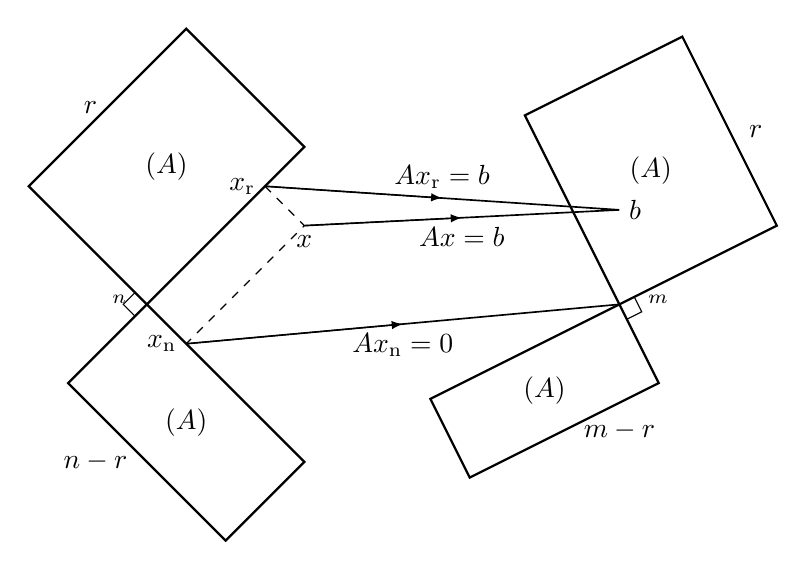
\begin{tikzpicture}
        \draw[thick](0, 0)node[left]{$\RR^n~$}--(2, 2)--(.5, 3.5)--(-1.5, 1.5)node[midway, left]{$r$}--(2, -2)--(1, -3)--(-1, -1)node[midway, left]{$n-r~$}--cycle;
        \draw(-.15, .15)--(-.3, 0)--(-.15, -.15);
        \node at(.25, 1.75){$\C(A\tp)$};
        \node at(.5, -1.5){$\N(A)$};
        \draw[thick](6, 0)node[right]{$~~\RR^m$}--(8, 1)--(6.8, 3.4)node[midway, right]{$~r$}--(4.8, 2.4)--(6.5, -1)--(4.1, -2.2)node[midway, right]{$~m-r$}--(3.6, -1.2)--cycle; % +6
        \draw(6.19, .095)--(6.285, -.095)--(6.095, -.19); % .03√10
        \node at(6.4, 1.7){$\C(A)$};
        \node at(5.05, -1.1){$\N(A\tp)$};
        \coordinate[label=below:$x$](X)at(2, 1);
        \coordinate[label=left:$x_\mathrm r$](R)at(1.5, 1.5);
        \coordinate[label=left:$x_\mathrm n$](N)at(.5, -.5);
        \coordinate[label=right:$b$](B)at(6, 1.2);
        \draw[dashed](R)--(X)--(N);
        \draw[semithick](R)--(B)--(X);
        \draw[semithick](N)--(6, 0);
        \draw[-latex](R)--(3.75, 1.35)node[above]{$Ax_\mathrm r=b$};
        \draw[-latex](X)--(4, 1.1)node[below]{$Ax=b$};
        \draw[-latex](N)--(3.25, -.25)node[below]{$Ax_\mathrm n=0$};
    \end{tikzpicture}
    \captionof{figure}{big picture升级版}
\end{center}
\section{投影}
考虑向量$b$在向量$a$上的投影$p$
\[
	p=(\hat a\cdot b)\hat a=\frac{a\tp b}{a\tp a}a=\frac{aa\tp}{a\tp a}b.
\]
考虑$\RR^m$中线性无关的$n$个向量$(a_1,\ldots,a_n)=:A$张成的子空间,找到向量$p$在上面的投影
\[
	p=Ax=x_1a_1+\cdots+x_na_n\in\C(A).
\]
考虑投影的性质:$p$的终点在子空间中距离$b$的端点最近,则$(b-p)$同子空间垂直:
\[
	A\tp(b-Ax)=0
\]
相当于求解线性方程组
\[
	A\tp Ax=A\tp b.
\]
若$A\tp A$可逆,则$x=(A\tp A)\iv A\tp b$,由$p=Ax$可定义投影矩阵(project matrix)
\begin{align}
	P=A(A\tp A)\iv A\tp.
\end{align}
投影矩阵有性质:$P^2=P$,这也是符合投影性质的。
\begin{theorem}{$A\tp A$的可逆性}{ATA inverse}
	$A\tp A$可逆$\iff A$的列之间线性无关。
\end{theorem}
\begin{proof}
	只需证明$\N(A\tp A)=\N(A)$即可。
	
	$\forall x\in\N(A),\enspace Ax=0$,左乘$A\tp$得:$A\tp Ax=0$,故$x\in\N(A\tp A)$;
	
	$\forall x\in\N(A\tp A),\enspace A\tp Ax=0$,左乘$x\tp$得:$x\tp A\tp Ax=\norm{Ax}^2=0$,因此$Ax=0$,故$x\in\N(A)$。
\end{proof}
\begin{corollary}
	\[
		\rank(A)=\rank(A\tp)=\rank(A\tp A)=\rank(AA\tp).
	\]
\end{corollary}

\section{最小二乘法}
考虑线性方程组$Ax=b$,$A$的行数$m>$列数$n$甚至$m\gg n$,一般来说无解。但仍可找到$x$使得$\norm{b-Ax}$最短。

由投影的性质,若$Ax$是$b$在$\C(A)$上的投影,则$\norm{b-Ax}$最短,此时
\[
	x=(A\tp A)\iv A\tp b.
\]
\begin{method}{直线拟合(最小二乘法)}{}
	$m$组数据$(x_i,y_i)$,确定线性关系$y=a+bx$中的系数$a,b$,即 
	\[
		\begin{bmatrix}
			1&x_1\\\vdots&\vdots\\1&x_m
		\end{bmatrix}
		\begin{bmatrix}
			a\\b
		\end{bmatrix}=
		\begin{bmatrix}
			y_1\\\vdots\\y_m
		\end{bmatrix},\iff Ax=b.
	\]
	\newcommand*{\sumi}[1]{\langle{#1}\rangle}
	$A$列满秩$\rank(A)=2$,故$A\tp A$可逆,
	\[
		A\tp A=
		\begin{bmatrix}
			m&\sumi{x_i}\\
			\sumi{x_i}&\sumi{x_i^2}
		\end{bmatrix},\quad
		(A\tp A)\iv=\frac1{m\sumi{x_i^2}-\sumi{x_i}^2}
		\begin{bmatrix}
			\sumi{x_i^2}&-\sumi{x_i}\\
			-\sumi{x_i}&m
		\end{bmatrix}.
	\]
	在此处$\sumi{\cdot}$特指对$i$求和,得到 
	\[
		\begin{cases}
			a=\frac{\sumi{x_i^2}\sumi{y_i}-\sumi{x_i}\sumi{x_iy_i}}{m\sumi{x_i^2}-\sumi{x_i}^2}\\
			b=\frac{-\sumi{x_i}\sumi{y_i}-m\sumi{x_iy_i}}{m\sumi{x_i^2}-\sumi{x_i}^2}
		\end{cases}
	\]
	\iffalse
	\[
		A\tp A=
		\begin{bmatrix}
			n&\textstyle\sum_{i=1}^n x_i\\
			\textstyle\sum_{i=1}^n x_i&\textstyle\sum_{i=1}^n x_i^2
		\end{bmatrix}
	\]
	则
	\[
		(A\tp A)\iv=\frac1{\textstyle{n\sum_{i=1}^n x_i^2-\bigkh{\sum_{i=1}^n x_i}^2}}
		\begin{bmatrix}
			\textstyle\sum_{i=1}^n x_i^2&-\textstyle\sum_{i=1}^n x_i\\
			-\textstyle\sum_{i=1}^n x_i&n
		\end{bmatrix}
	\]
	得到 
	\[
		\begin{cases}
			a=\frac{\textstyle\sum_{i=1}^n x_i^2\sum_{i=1}^n y_i-\sum_{i=1}^n x_i\sum_{i=1}^n x_iy_i}{\textstyle{n\sum_{i=1}^n x_i^2-\bigkh{\sum_{i=1}^n x_i}^2}}\\[2ex]
			b=\frac{\textstyle-\sum_{i=1}^n x_i\sum_{i=1}^n y_i-n\sum_{i=1}^n x_iy_i}{\textstyle{n\sum_{i=1}^n x_i^2-\bigkh{\sum_{i=1}^n x_i}^2}}
		\end{cases}
	\]
	\fi
\end{method}
\begin{method}{多项式拟合}{}
	$m$组数据$(x_i,y_i)$,确定多项式关系
	\[
		y=a_0+a_1x+\cdots+a_nx^n
	\]
	中的系数$a_0,\ldots,a_n$,即 
	\[
		\begin{bmatrix}
			1&x_1&\cdots&x_1^n\\\vdots&\vdots&\ddots&\vdots\\1&x_m&\cdots&x_m^n
		\end{bmatrix}
		\begin{bmatrix}
			a_0\\\vdots\\a_n
		\end{bmatrix}=
		\begin{bmatrix}
			y_1\\\vdots\\y_m
		\end{bmatrix},\iff Ax=b.
	\]
	从而$x=(A\tp A)\iv A\tp b.$
\end{method}
% 一般最小二乘拟合:……

\begin{remark}
	两组数据相关不一定代表有因果。
\end{remark}

\section{正交归一基}

基是一组线性无关的向量并且张成整个线性空间,我们对基之间的夹角和长度并没有要求。为了方便,我们可以要求基具备一些额外的性质。
\begin{definition}{正交归一基}{orthonomal basis}
	基$\{q_1,\ldots,q_n\}$是正交归一的(orthonomal)的,若 
	\[
		q_i\cdot q_j=\delta_{ij}
	\]
\end{definition}
将一组正交归一基$\{q_1,\ldots,q_n\}$按列排成矩阵$Q$,则$Q\tp Q=I$,称为正交矩阵(orthogonal matrix)。特别的,若$Q$是方阵,则
\[
	Q\tp=Q\iv,
\]
则$Q\tp Q=QQ\tp=I$,便得到正交归一基的完备性(completeness)
\[
	\sum_{i=1}^nq_iq_i\tp=I.
\]
\begin{example}{Fourier级数}{Fourier series}
	定义函数$f,g$在$[-\pi,\pi]$上的内积
	\[
		\inp fg:=\int_{-\pi}^\pi f(x)g(x)\d x
	\]
	则三角函数系列
	\[
		\hkh{\frac1{\sqrt{2\pi}},\frac{\sin\theta}{\sqrt\pi},\frac{\cos\theta}{\sqrt\pi},\frac{\sin2\theta}{\sqrt\pi},\frac{\cos2\theta}{\sqrt\pi},\ldots}
	\]
	构成一组正交归一基,任意$[-\pi,\pi]$上平方可积的函数均可被展开为Fourier级数(Fourier series):
	\[
		f(x)=\frac{a_0}2+\sum_{n=1}^\infty(a_n\cos nx+b_n\sin nx).
	\]
	Fourier系数
	\[
		\begin{cases}
			a_n:=\frac1\pi\int_{-\pi}^\pi f(x)\cos nx\d x\\
			b_n:=\frac1\pi\int_{-\pi}^\pi f(x)\sin nx\d x
		\end{cases}
	\]
\end{example}

\subsection{Gram-Schmidt法则}

给定一组基$\{a_1,\ldots,a_n\}$,如何构造一组正交归一基$\{q_1,\ldots,q_n\}$?
\begin{method}{Gram-Schmidt法则}{Gram-Schmidt rule}
	\begin{compactenum}
		\item 选取$b_1:=a_1;$
		\item 从$a_2$减去沿着$b_1$方向的分量,作为$b_2$
		\[
			b_2:=a_2-\frac{b_1\tp a_2}{b_1\tp b_1}b_1;
		\]
		\item 从$a_i$减去沿着$b_1,\ldots,b_{i-1}$方向的分量,作为$b_i$
		\[
			b_i:=a_i-\sum_{j=1}^{i-1}\frac{b_j\tp a_i}{b_j\tp b_j}b_j.
		\]
	\end{compactenum}
	再归一化$\{b_1,\ldots,b_n\}$
	\[
		q_i:=\frac{b_i}{\norm{b_i}}.
	\]
\end{method}

\subsection{\texorpdfstring{$QR$}{QR}分解}

\begin{theorem}{QR分解}{QR decomposition}
	若$m\times n$矩阵$A=(a_1,\ldots,a_n)$的列之间线性无关,可用Gram-Schmidt法则构造一组正交归一基$\{q_1,\ldots,q_n\}$,$q_i$同$a_1,\ldots,a_{i-1}$正交,定义
	\[
		R:=Q\tp A=\begin{bmatrix}
			q_1\tp a_1&q_1\tp a_2&\cdots&q_1\tp a_n\\[1ex]
			0&q_2\tp a_2&\cdots&q_2\tp a_n\\
			0&0&\ddots&\vdots\\
			0&0&0&q_n\tp a_n
		\end{bmatrix}
	\]
	$R$是个上三角矩阵,故$A$可以写成正交矩阵和上三角矩阵的乘积:
	\begin{equation}
		A=QR.
	\end{equation}
\end{theorem}

在最小二乘法等应用中,$A\tp A=R\tp R$
\[
	x=(A\tp A)\iv A\tp b=R\iv Q\tp b.
\]
效率更高。
